% -------------------------------------------------------------------------------------------------
% Definitionen
% -------------------------------------------------------------------------------------------------
\documentclass[
    fontsize=12pt,                      % Schriftgröße 12 pt
    paper=a4,                           % Seitengröße A4
    twoside=off,                       % zweiseitiger Druck
    DIV=15,                             % Seiteneinteilung
    BCOR=12mm,                          % Bindekorrektur
    headings=normal,                    % normal große Überschriften
    headsepline=false,                   % Trennlinie unter der Kopfzeile
    footsepline=false,                  % Trennlinie über der Fußzeile
    headinclude=true,                   % Kopfzeile zählt zum Textkörper
    footinclude=false,                  % Fußzeile zählt nicht zum Textkörper
    toc=listof,                         % Verzeichnisse der Gleitumgebungen ins Inhaltsverzeichnis
    toc=bib,                            % Literaturverzeichnis ins Inhaltsverzeichnis
    chapterprefix=false,                % vor Kapitelnummern steht "Kapitel"
    appendixprefix=false,               % vor Anhangüberschriften steht "Anhang"
    numbers=noendperiod,                % Keinen Punkt hinter die letzte Zahl eines Kapitels (auch bei Anhang)
    captions=tableabove,                % Tabellenüberschriften setzen
    footnotes=multiple,                 % Erkennung von mehreren Fußnoten hintereinander
    bibliography=oldstyle,              % Literaturverzeichnis: openstyle oder oldstyle
    draft=false,                        % Entwurfsstadium
]{scrreprt}


% Paket Includes
% ----------------------------
\usepackage[T1]{fontenc}                % deutsche Umlaute und Sonderzeichen
\usepackage[utf8]{inputenc}             % Umlaute koennen direkt im Quelltext stehen
\usepackage[ngerman]{babel}             % neue deutsche Rechtschreibung 
\usepackage{lmodern}
\usepackage{graphicx}                   % Bilder einfügen
\usepackage{tabularx}                   % Tabellen mit fester Breite und variabler Spaltenbreite
\usepackage{array,longtable}            % Tabellen mit Seitenumbruch
\usepackage{booktabs}                   % bessere horizontale Linien in Tabellen
\usepackage{array,ragged2e}             % mehr Spaltentypen in Tabellen und neue Spaltentypen
\usepackage{dcolumn}                    % Spalten am Dezimaltrenner ausrichten
\usepackage{amsmath}
\usepackage[                            % Unterabbildungen mit folgenden Parametern:
            font=footnotesize,          % kleine Schrift
            labelfont={sf,bf},          % Labels fett und serifenlos
            textfont={sf},              % Text serifenlos
            format=hang,                % hängender Einzug
           ]{caption}
\usepackage{float}      
\usepackage{hyperref}                   % URL links  
\usepackage{xcolor}  
\usepackage{listings}

\definecolor{mygreen}{rgb}{0,0.6,0}
\definecolor{myred}{rgb}{0.7529,0.3137,0.3019}


\newcommand{\Farbcode}[1]{\texttt{\textbf{\textcolor{myred}{#1}}}}
   

% Kopf- und Fußzeile
% ----------------------------
\usepackage{scrlayer-scrpage} 
\setkomafont{pagehead}{\sffamily\small}
\setkomafont{pagefoot}{\sffamily\small}
%\automark{chapter}
\lohead{Modul Embedded Systems 2 -- Steuergeräte, Vernetzung, Software} \cohead{} \rohead{Übung 3-3}
\lofoot{\includegraphics[height=10pt]{Figures/HSMW-Logo-klein} HS Mittweida, INW, Prof. Thomanek}
\cofoot{} \rofoot{\thepage}

\pagestyle{headings}
\renewcommand*{\chapterpagestyle}{headings}% Nicht zu empfehlen, aber du willst das offenbar trotzdem.


\setcounter{secnumdepth} {3}
\addto\captionsngerman{\renewcommand{\figurename}{Abb.}}    % Verwende Abb. x.x anstatt Abbildung x.x
\renewcommand{\thefigure}{\arabic{figure}}
% -------------------------------------------------------------------------------------------------
% Dokument
% -------------------------------------------------------------------------------------------------

\begin{document}


\chapter*{Übung 3-3 C++-Programmierung -- \\Klassendefinition}

\section*{1. Implementierung einer Matrix-Klasse}
Implementieren Sie die Klasse \Farbcode{CMatrix} für Matrizenberechnungen. 
\vskip 0.2cm 
\noindent \textbf{Es gelten folgende Anforderungen:}
\begin{itemize}
\item Der \textbf{Datentyp} der Matrix ist \texttt{double}
\item Die \textbf{Dimension} der Matrix beträgt fest 3x3
\item Neben dem \textbf{Standard-Konstruktor} soll es folgende weitere \textbf{Konstruktoren} geben
\begin{itemize}
\item mit Übergabe eines Skalar für die Initialisierung der Matrixelemente
\item mit Übergabe eines Datenfeldes für die Initialisierung der Matrixelemente
\item mit Übergabe einer Matrix (Copy-Konstruktor)
\end{itemize}
\item Folgende \textbf{Methoden} sind zu implementieren:
\begin{itemize}
\item Ein bestimmtes Element lesen und setzen
\item Addition und Multiplikation mit einem Skalar
\item Addition/Subtraktion zweiter Matrizen 
\item Transponieren 
\item Optional: Multiplikation zweier Matrizen

\end{itemize}
\end{itemize}
 
\vskip 1cm

\section*{2. Test der Matrixoperationen}
Implementieren Sie Testroutinen, um die Matrixklasse zur testen. Vergleichen Sie die Ergebnisse mit dem Taschenrechner bzw. mithilfe von MATLAB.  
\newpage
\section*{3. Erstellen einer LED-Klasse für den Arduino}
Implementieren Sie eine Klasse \Farbcode{CLed} (\texttt{CLed.h, CLed.cpp}) zur Kapselung/Abstraktion der Ansteuerung einer LED am Arduino UNO.
\vskip 0.2cm 
\noindent \textbf{Es gelten folgende Anforderungen:}\begin{itemize}
\item Konstruktor mit Übergabe Port, Bit-Position und Flag bzgl. LED-Anschluss (gegen $U_B$ oder Masse) -- (Default-Konstruktor verwendet Onboard-LED))
\item Methode zum Einschalten der LED \Farbcode{On()}
\item Methode zum Ausschalten der LED \Farbcode{Off()}
\item Methode zum Abfragen des aktuellen Status \Farbcode{IsOn()}
\item Methode zum Wechseln des LED-Stati \Farbcode{Toggle()}
\end{itemize}
\vskip 0.2cm 
\noindent \textbf{Hinweise:}
\begin{itemize}
\item Die Adressen der \emph{Portregister} sind: Port B: \Farbcode{0x25}, Port C: \Farbcode{0x28}, Port D: \Farbcode{0x2B} bzw. die Adressen für \emph{Data Direction Register} lauten: Port B: \Farbcode{0x24}, Port C: \Farbcode{0x27}, Port D: \Farbcode{0x2A}
\item Berücksichtigen Sie nur Ports bzw. Pin-Nummern die gemäß Arduino-Board (siehe Bild) unterstützt werden
\end{itemize}

\begin{figure}[H]
	\centering
	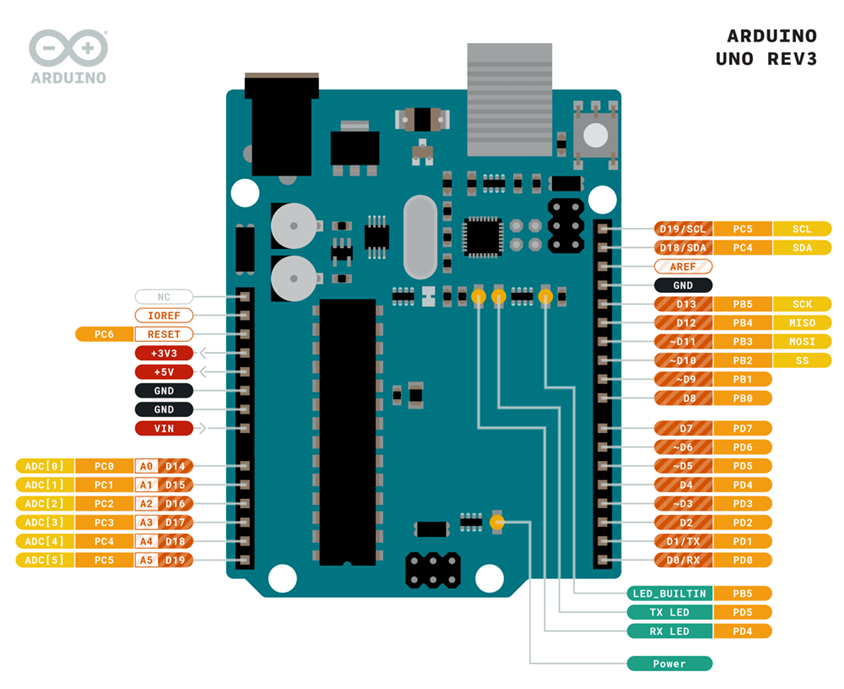
\includegraphics[width=0.7\textwidth]{Figures/arduino}
\end{figure}
\noindent
\textbf{Testen Sie} die Klasse, indem Sie im Sketch ein Objekt der Klasse \Farbcode{CLed} anlegen und es entsprechend der erstellten Methoden geeignet verwenden.
\end{document}


